\chapter{Периферийная и внутренняя конфигурации модельной сборки ТВЭЛов}\label{ch:ch4}

\section{Постановка задачи}\label{ch4:problem}

%
%
\begin{figure}[h!]
  \centering
  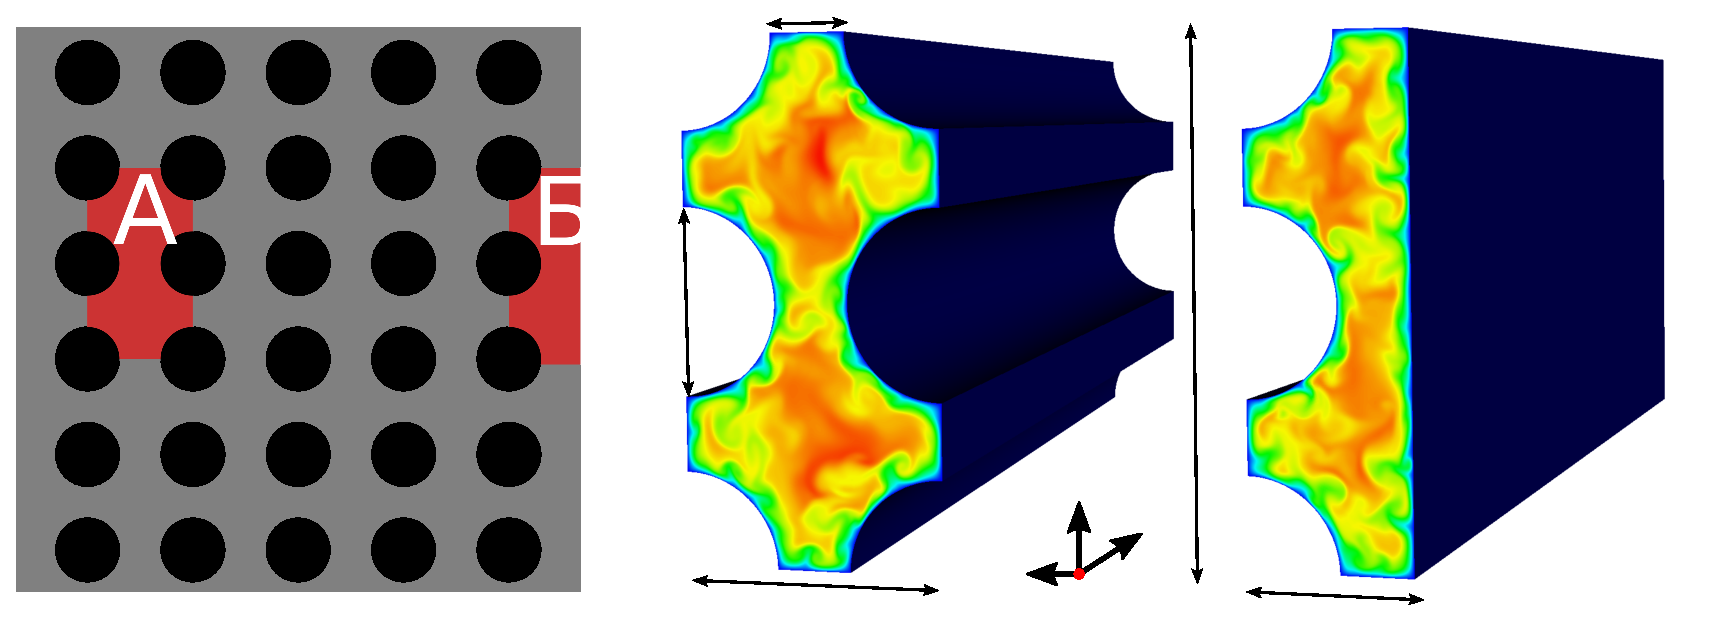
\includegraphics[width=0.9\textwidth]{fig1_new.eps}
  \caption{Модель тепловыделяющей сборки с геометрическими размерами. 
  Черным цветом показаны ТВЭЛы, серым -- теплоноситель. Область типа А -- внутренняя, 
  типа Б -- периферийная}
  \label{fig:1}
\end{figure}
%

%
На Рисунке \ref{fig:1} показаны геометрические модели для расчета двух типов ТВЭЛов: 
6-ти внутренних и 3-х периферийных.
%
Диаметр и шаг расположения ТВЭЛов в обоих случаях одинаковы.
%
В дальнейшем условимся обозначать продольное, горизонтальное и 
вертикальное направления как $(x,y,z)$, соответственно.
%
ТВЭЛы представляют собой цилиндры радиуса 5 мм. с вертикальным и 
горизонтальным зазорами по 4 мм. между собой. 
%
Размер в продольном направлении составляет 140 мм., так что продольные когерентные 
вихревые структуры целиком умещаются в рассматриваемую область.
%
В дальнейшем все результаты приводятся в безразмерном виде, где координаты нормированы 
на высоту модели ($H=28$ мм.), а скорость на среднерасходную скорость $U_b$.
%


В задаче рассматривается течение жидкости при фиксированном числе 
Рейнольдса \textit{Re~}$ = 13000$, построенному по гидравлическому диаметру и среднерасходной скорости.
%
Динамика течения полностью описывается уравнениями Навье-Стокса в несжимаемой постановке:
\begin{equation}\label{n-stoks:dimen}
\pfrac{u_i}{t} + u_j \pfrac{u_i}{x_j}= - \pfrac{p}{x_i} + \frac{1}{Re} \pfrac{\tau_{ij}}{x_j},
\end{equation}
%
где $u_i$ - $i$-ая компонента вектора скорости ($i={1,2,3}$), $x_j$ - $j$-ая координата,
%
\begin{equation*}\label{stress:tensor}
\tau_{ij} = \pfrac{u_i}{x_j} + \pfrac{u_j}{x_i}
\end{equation*}
обозначает тензор вязких напряжений.
%
Все величины обезразмерены на характерные значения.
%
$Re = U_b D_h/\nu$ обозначает число Рейнольдса, построенное по среднерасходной скорости 
и гидравлическому диаметру.

%
Используется два типа граничных условий (ГУ): стенка и периодическое направление.
%
На стенках используется условие прилипания для поля скорости ($u_i = 0$), 
а также отсутствие поперечного градиента давления ($dp/dn = 0$). 
%
В продольном направлении используются периодические граничные условия для моделирования достаточно длинной ТВС.


%
Для численного решения уравнений (\ref{n-stoks:dimen}) используется открытый вычислительный код Nek5000, р
азработанный Полом Фишером и др. \cite{nek}.
%
Валидация численных алгоритмов была проведена нами ранее на примере различных задач гидродинамики 
\cite{zaripov2021mechanism,zaripov2021reverse,ivashchenko2021effect}.
%
В его основе лежит метод спектральных элементов (SEM, от англ. Spectral Element Method), 
по принципу работы схожий с широко известным методом конечных объемов, 
но в котором решение и данные представлены в виде разложения по многочленам $N$-го порядка
в каждом из $E$ деформируемых гексагональных элементов.
%
Обычно $N$ варьируется от 8 до 16, так как при использовании меньшего значения $N$ 
не используются преимущества SEM, а большие значения использовать дорого с вычислительной точки зрения. 
%
В данной работе  $N=10$.
%
SEM отличается малой величиной численной дисперсии и диссипации, 
что является важным при расчете эволюции гидродинамических неустойчивостей, а также высоких числах Рейнольдса.
%
Спектральная точность означает экспоненциальное уменьшение ошибки с ростом количества вычислительных узлов.
%
Дискретизация по времени происходит при помощи формулы ``дифференцирования назад'' 3-го порядка точности.
%
В рамках пространственной дискретизации в каждом из $E$ элементов переменные 
задачи раскладываются по базису ${\psi_i}$, состоящему из интерполяционных полиномов Лагранжа:
%
\[
\psi_i(x)=\prod_{j \neq i}\frac{x-\xi_j}{\xi_i-\xi_j}, 
\]
%
где $\xi_i$ - точки, являющиеся корнями уравнения:
\[
(1-\xi^2)\frac{d}{d\xi}P_N(\xi)=0,
\]
в котором $P_N$ - полиномы Лежандра порядка $N$. 
%
Иными словами, $\xi_i$ определяют положение точек сетки внутри спектрального элемента.
%
Более подробно алгоритмы дискретизации и решения уравнений в коде Nek5000 ранее были описаны в Главе 1.
%

%
\begin{figure}[h!]
  \centering
  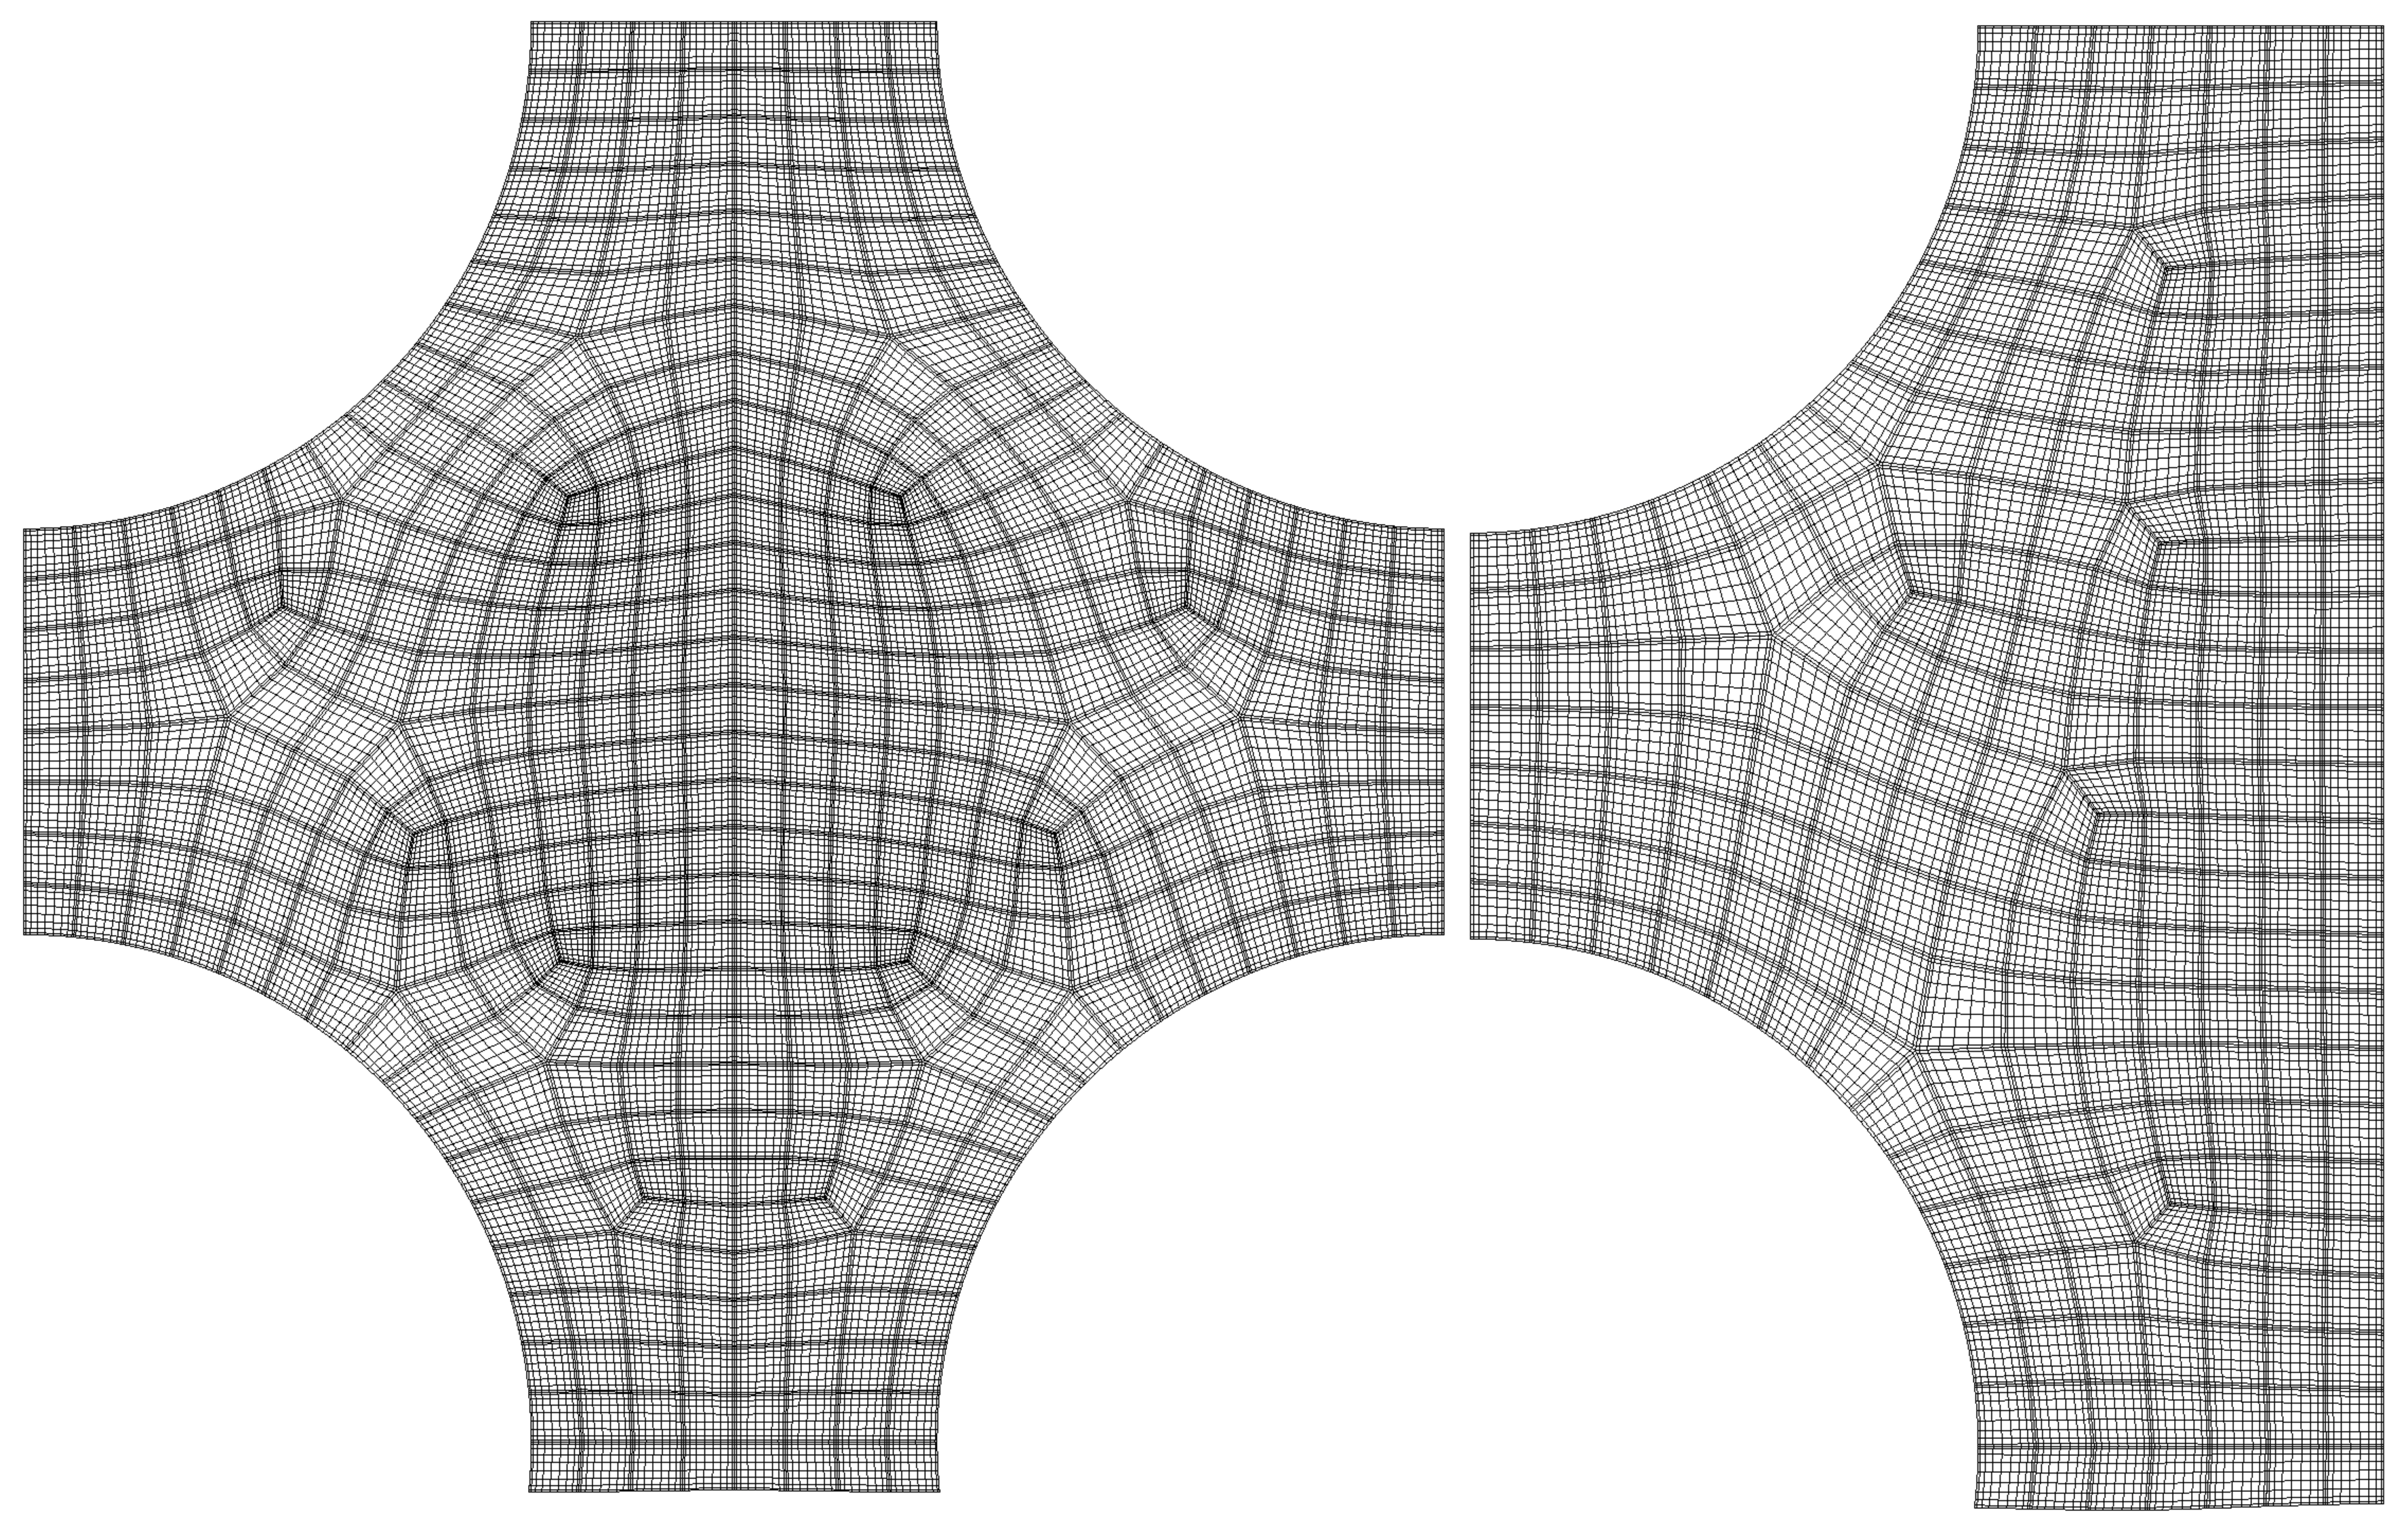
\includegraphics[width=0.5\textwidth]{mesh.eps}
  \caption{Пример вычислительной сетки для поперечного сечения верхней половины геометрии}
  \label{fig:3}
\end{figure}



Вычислительная сетка состоит из порядка 40 млн. узлов для внутренней 
и 18 млн. узлов для периферийной конфигураций (см. Рисунок \ref{fig:3}).
%
Дополнительно была проверена сеточная сходимость для уверенности в достоверности получаемых данных.
%
Также была произведена оценка отношения наименьшего размера вихрей (колмогоровского масштаба)  
$\eta_k = (\nu^3/\epsilon)^\frac{1}{4}$, где $\nu$ -- кинематическая вязкость, 
$\epsilon$ -- скорость диссипации, к шагу сетки $\Delta$.
%
Минимальный шаг сетки оказался сопоставим с колмогоровским масштабом 
$\Delta_{min} \approx \eta_k$, а максимальный шаг сетки превысил его всего лишь в 3 раза 
$\Delta_{min} \approx 3\eta_k$, что является хорошим показателем качества вычислительной сетки.


\section{Результаты}\label{ch4:results}

\begin{figure}[h!]
  \centering
  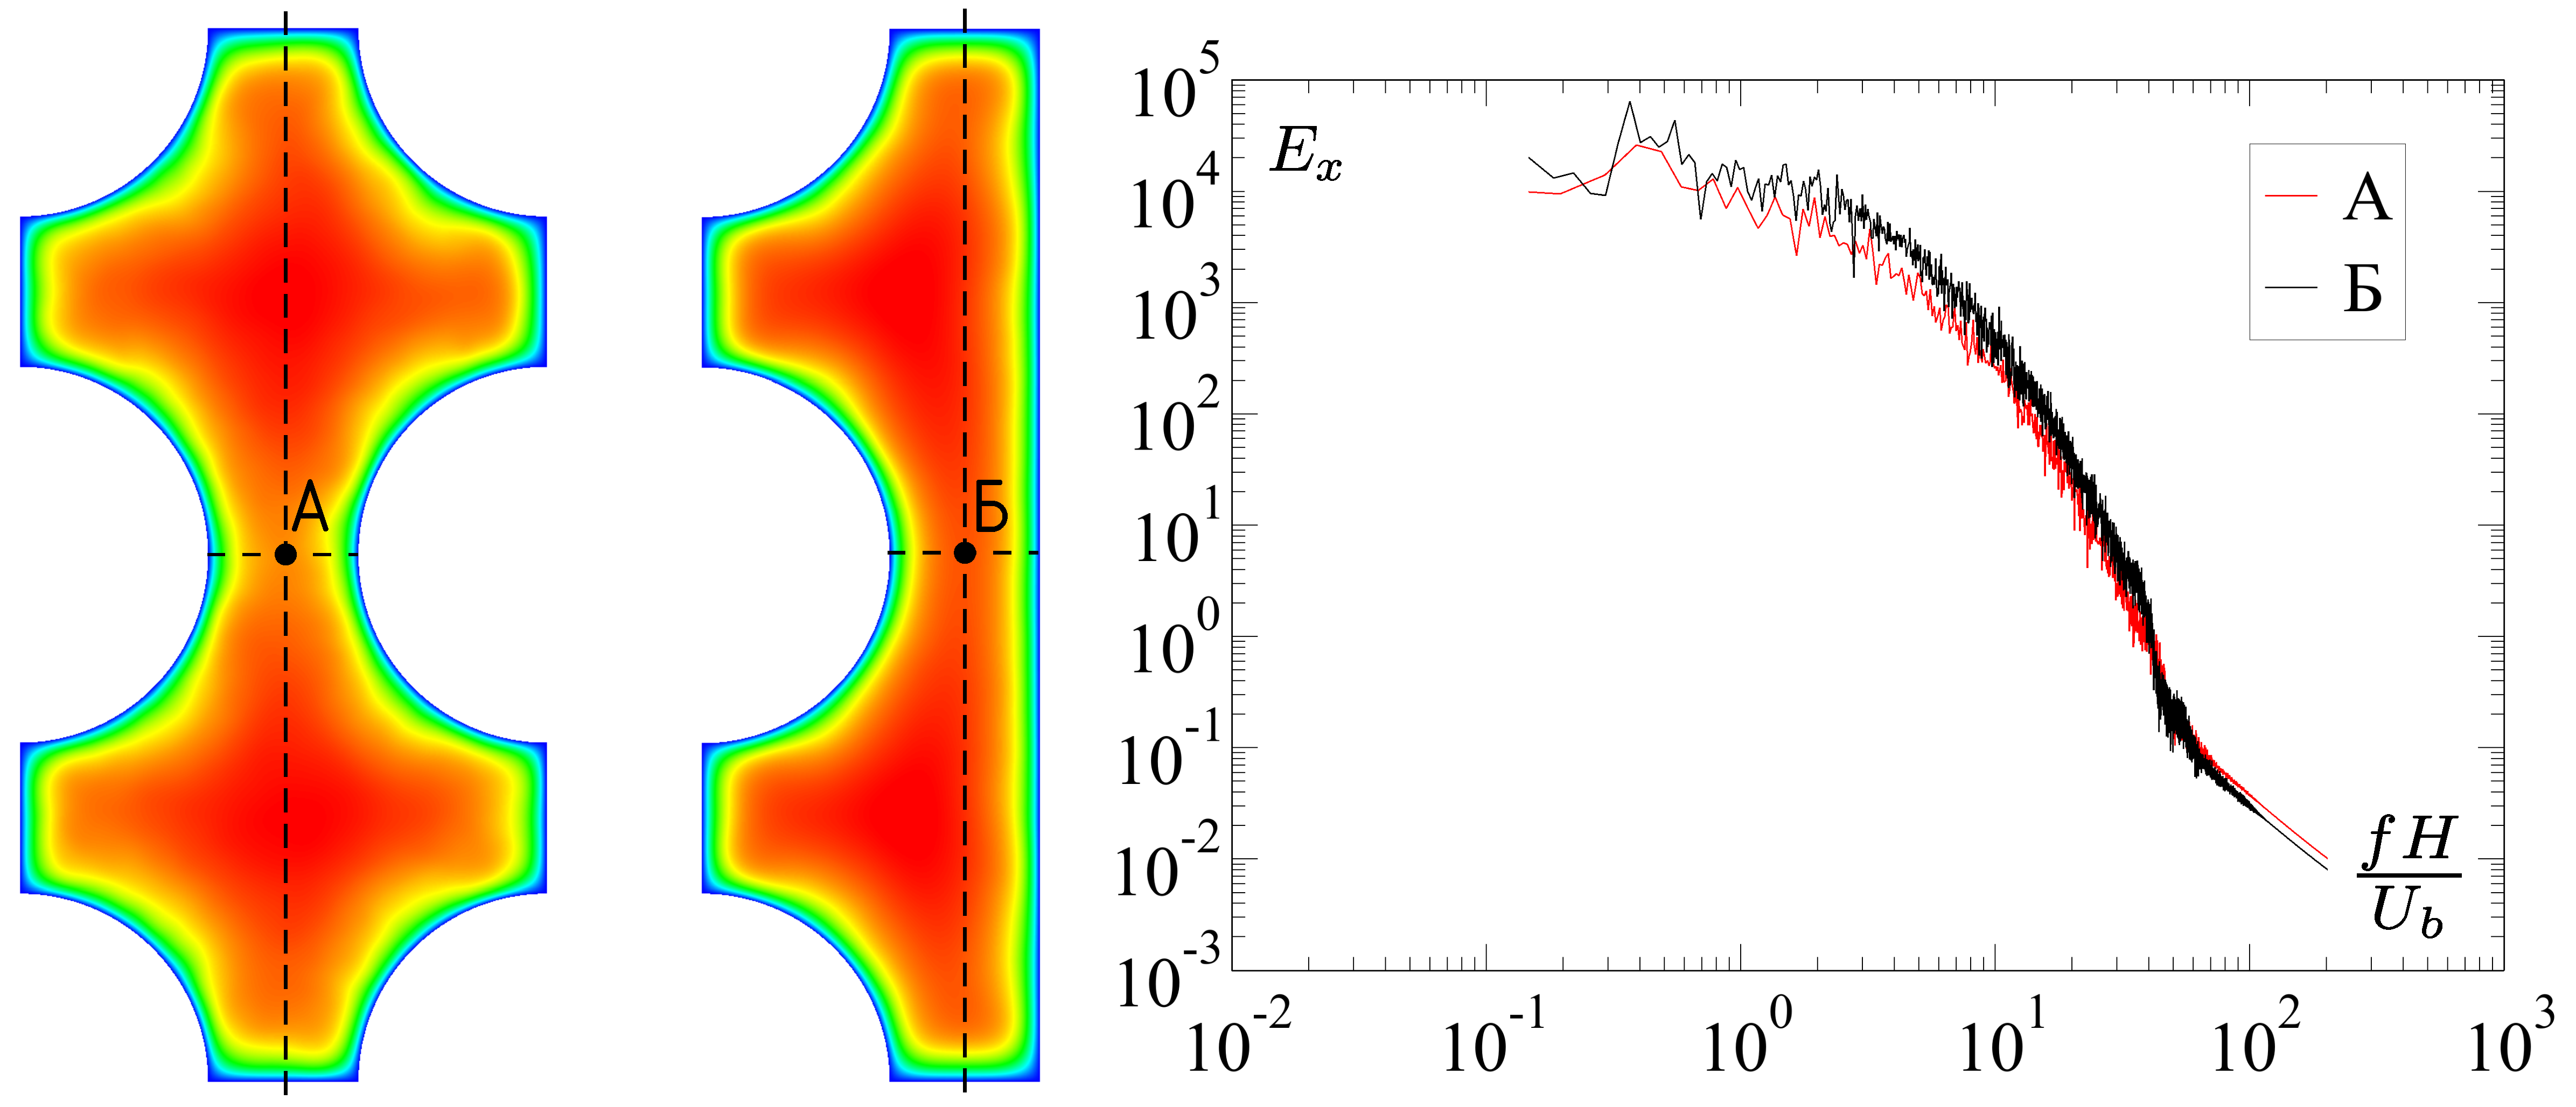
\includegraphics[width=0.9\textwidth]{spectres.eps}
  \caption{Спектры турбулентной кинетической энергии для двух конфигураций. 
  Пунктирными линиями показаны сечения, в которых сравниваются средние профили 
  скорости и пульсаций на Рисунке \ref{fig:5}}
  \label{fig:4}
\end{figure}


На Рисунке \ref{fig:4} показано сравнение спектров турбулентной кинетической энергии 
продольной компоненты скорости ($E_x(fH/U_b)$) в центральных точках обоих конфигураций (отмечены на рисунке). 
%
Турбулентная кинетическая энергия получается с помощью процедуры 
быстрого преобразования Фурье (FFT, от англ. Fast Fourier Transform): 
$E_x = |FFT(u'_x)^2|$, где $u'_x = u_x - \overline{u_x}$ -- мгновенные пульсации продольной скорости, 
а $\overline{u_x}$ -- осредненное по времени поле продольной скорости. 
%
В качестве аргумента используется безразмерная частота $fH/U_b$.

%
Стоит отметить, что в спектрах присутствуют несколько пиков, соответствующих выделенным частотам. 
%
Наличие выделенных частот в потоке соответствует поперечным колебаниям скорости в зазоре, 
которые связаны с развитием вихревых структур. 
%
Несмотря на то, что в обоих случаях наблюдаются близкие безразмерные частоты, 
в спектрах уровень кинетической турбулентной энергии выше в случае периферийной конфигурации.
%
При этом на Рисунке \ref{fig:4} пунктирными линиями также показаны горизонтальное и вертикальное сечения, 
в которых проводилось сравнение профилей средней продольной скорости и ненулевых компонент тензора 
напряжений Рейнольдса, показанное на Рисунке \ref{fig:5}.
%
Видно, что для обоих случаев спектры очень близки, при этом характерные безразмерные частоты на спектре также 
отличаются незначительно: 0.39 для внутренней конфигурации и 0.37 для периферийной. 
%


\begin{figure}[h!]
  \centering
  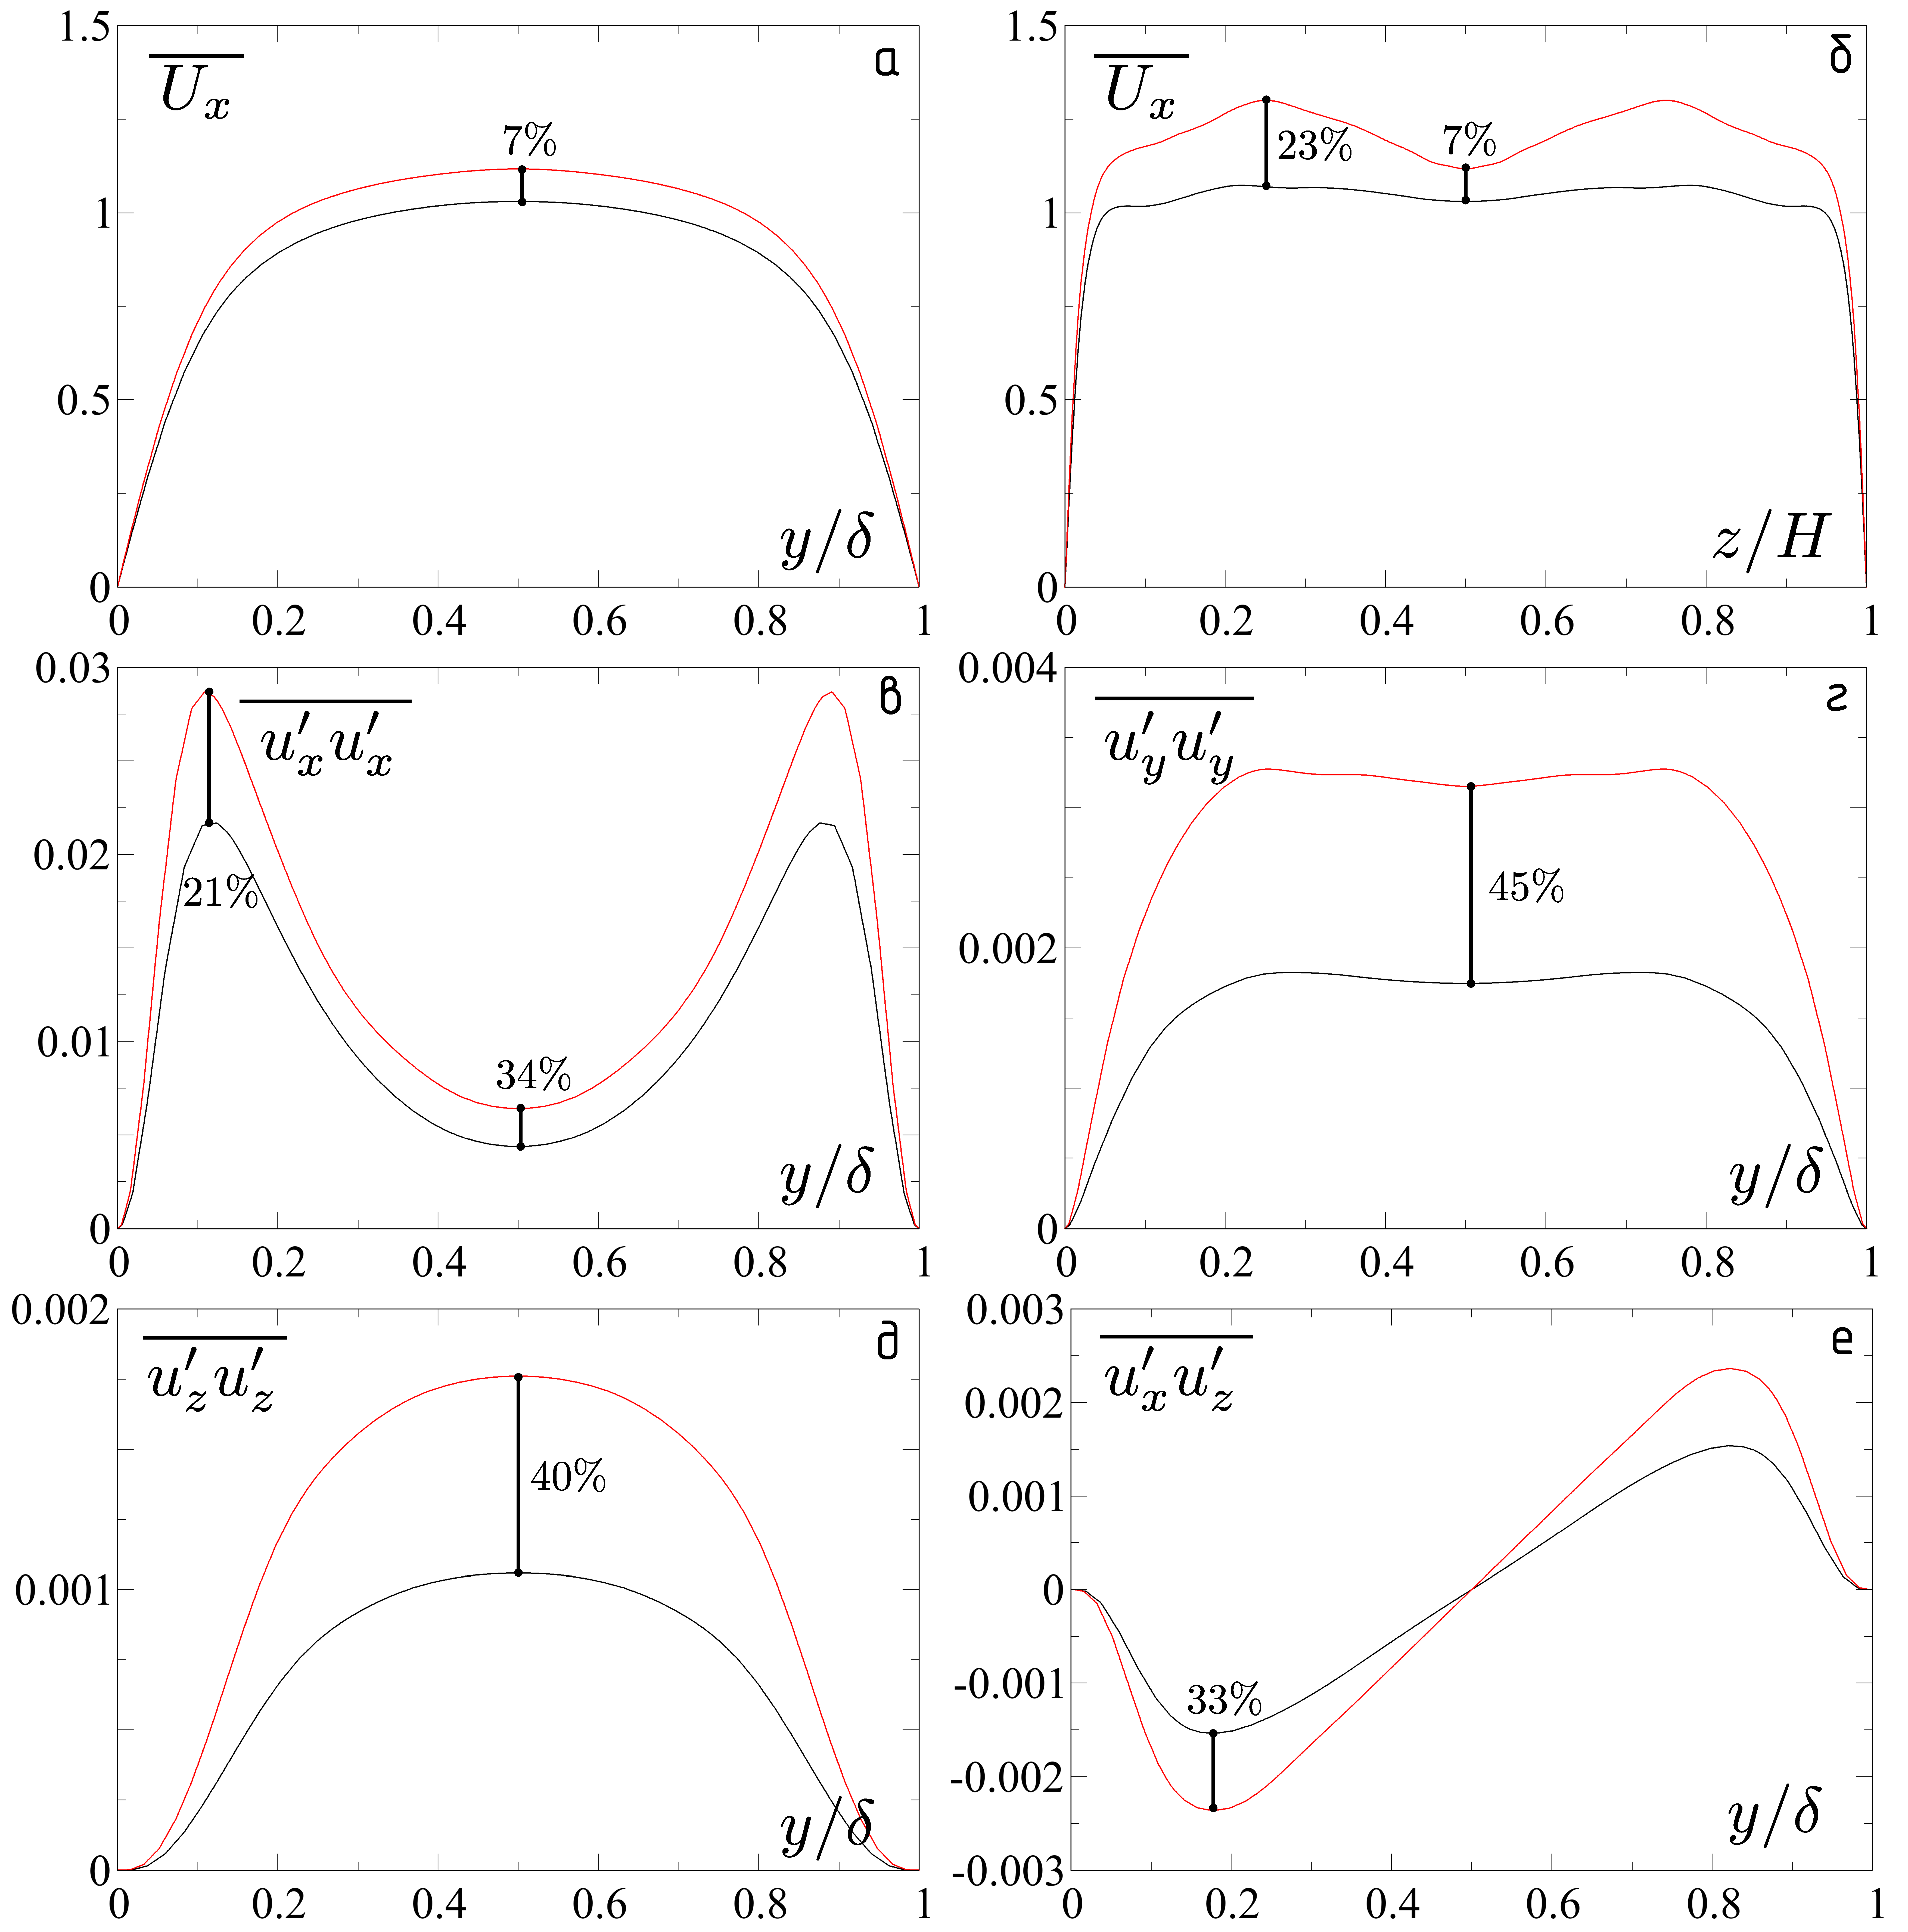
\includegraphics[width=0.9\textwidth]{profiles_mid.eps}
  \caption{Профили ненулевых компонент тензора напряжений Рейнольдса и средней продольной скорости для двух рассмотренных конфигураций. Красным цветом показаны результаты для внутренней сборки, черным -- для периферийной. Горизонтальная ось соответствует расстоянию $y/H$ вдоль пунктирной линии, показанной на Рисунке \ref{fig:4}}
  \label{fig:5}
\end{figure}


%
%
%
На Рисунке \ref{fig:5}\textit{а} и \ref{fig:5}\textit{б} приведен профиль продольной 
скорости вдоль горизонтального и вертикального сечения, соответственно.
%
Горизонтальная координата нормирована на ширину межтвэльного пространства 
$\delta = 4$ мм., вертикальная -- на высоту модели $H = 28$ мм.
%
В межтвэльном пространстве наблюдается неплохое совпадение результатов 
(с точностью до 7\%), хотя в точках $z/H = 0.25$ и $z/H = 0.75$ наблюдается наибольшее различие 
в графиках из-за наличия плоской стенки в периферийной конфигурации и, как следствие,
 изменения структуры вторичных течений.
%
На рисунках \ref{fig:5}\textit{в} -- \ref{fig:5}\textit{е}, 
несмотря на довольно высокое отклонение профилей друг от друга, 
наблюдается качественное совпадение профилей для обоих конфигураций.
%
При этом стоит отметить, что наибольшие отклонения наблюдаются для наименее интенсивных 
компонент тензора напряжений Рейнольдса, которые вносят наименьший вклад в общую турбулентную 
кинетическую энергию.





\section{Выводы}\label{ch4:conclusion}
%
Было проведено прямое численное моделирование двух модельных областей сборок ТВЭЛов: внутренней и периферийной. 
%
Выявлено, что профили средней скорости, а также компонент тензора напряжений 
Рейнольдса имеют качественные сходства для обоих конфигураций. 
%
Наибольшие отклонения наблюдаются в наименее интенсивных компонентах 
тензора напряжений Рейнольдса, вследствие чего на спектре турбулентной 
кинетической энергии явных различий выявлено не было,
 что дает возможность предполагать о незначительном влиянии плоской стенки на 
 процессы переноса энергии в межтвэльном пространстве. 
%
При этом основные отличия между конфигурациями вызваны изменением 
структуры вторичных течений (для внутренней области они намного интенсивнее), 
что и приводит к изменению пульсационных характеристик.
%
Таким образом можно установить, что экспериментальные результаты при 
исследовании периферийной области сборки ТВЭЛов качественно отражают картину 
турбулентного течения и для внутренней части сборки, однако влияние найденных различий
 в профилях компонент тензора напряжений Рейнольдса на процессы теплопереноса 
 требует дальнейшего детального изучения.

